% !TeX root = ../main.tex
\section{Results and Discussion}
\label{sec:results}

\subsection{Calibration and Residual Prediction Performance}
\label{subsec:prediction_performance}

Physical calibration makes the aerodynamic model more consistent with the real
vehicle. On the held-out test split, force RMSE decreases from $6.64$ to
$5.42~\mathrm{N}$ for $f_{x,b}$, from $6.11$ to $3.52~\mathrm{N}$ for
$f_{y,b}$, and from $18.43$ to $13.10~\mathrm{N}$ for $f_{z,b}$. Moment RMSE
also decreases, from $0.152$ to $0.071~\mathrm{N\,m}$ for $m_{x,b}$, from
$1.285$ to $0.602~\mathrm{N\,m}$ for $m_{y,b}$, and from $0.211$ to
$0.102~\mathrm{N\,m}$ for $m_{z,b}$. This confirms that the calibrated
aerodynamic model is meaningful, while also showing that a large real-flight
residual remains.

Table~\ref{tab:residual_overall_results} compares the calibrated aerodynamic
model, direct black-box prediction, and neural corrections. The calibrated model
has an overall RMSE of $5.965$ on the sequence-aligned held-out rows. Adding a
residual MLP reduces RMSE to $2.481$, showing that instantaneous variables
explain a substantial part of the residual. The channel-aware hybrid Transformer
further reduces RMSE to $0.870$ and MAE to $0.443$, while using residual
correction for forces and direct prediction for moments. The direct Transformer
reaches a similar RMSE of $0.888$. These results show that the hybrid
formulation keeps black-box-level predictive accuracy while retaining an explicit
calibrated aerodynamic model for the force residual analysis below.

\begin{table}[t]
\centering
\caption{Held-out test comparison. Values are computed on each model's aligned test rows.}
\label{tab:residual_overall_results}
\resizebox{\columnwidth}{!}{%
\begin{tabular}{@{}lccc@{}}
\toprule
Method & Rows & RMSE & MAE \\
\midrule
Calibrated aerodynamic model & 58639 & 5.965 & 2.961 \\
Direct Transformer & 58639 & 0.888 & 0.455 \\
Calibrated model + residual MLP & 60671 & 2.481 & 1.286 \\
Channel-aware hybrid Transformer & 58639 & \textbf{0.870} & \textbf{0.443} \\
\bottomrule
\end{tabular}%
}
\end{table}

Target-wise results in Table~\ref{tab:residual_target_results} show that the
largest absolute improvements occur in the main force channels. For $f_{x,b}$,
RMSE decreases from $5.416$ to $0.780~\mathrm{N}$; for $f_{z,b}$, it decreases
from $13.091$ to $1.581~\mathrm{N}$. The side-force channel remains the hardest
force component, with $\mathrm{RMSE}/\sigma_y=0.828$, but still improves from
$3.521$ to $1.196~\mathrm{N}$. For the
moment channels, direct neural prediction is more appropriate than residual
correction to the calibrated moment output. The channel-aware model reduces
moment RMSE to $0.0021$, $0.0012$, and $0.00033~\mathrm{N\,m}$ for
$m_{x,b}$, $m_{y,b}$, and $m_{z,b}$, respectively, with positive $R^2$ in all
three channels.

\begin{table}[t]
\centering
\caption{Target-wise held-out test metrics for the calibrated aerodynamic model and channel-aware hybrid Transformer. $\sigma_y$ is the standard deviation of the held-out target channel. For force channels, the hybrid model uses calibrated-model residual correction; for moment channels, it uses direct prediction.}
\label{tab:residual_target_results}
\resizebox{\columnwidth}{!}{%
\begin{tabular}{@{}lcccccc@{}}
\toprule
Target & $\sigma_y$ & Model RMSE & Hybrid RMSE & RMSE/$\sigma_y$ & Hybrid MAE & Hybrid $R^2$ \\
\midrule
$f_{x,b}$ & 4.826 & 5.416 & 0.780 & 0.162 & 0.592 & 0.974 \\
$f_{y,b}$ & 1.445 & 3.521 & 1.196 & 0.828 & 0.866 & 0.315 \\
$f_{z,b}$ & 9.294 & 13.091 & 1.581 & 0.170 & 1.197 & 0.971 \\
$m_{x,b}$ & 0.00332 & 0.0716 & 0.00210 & 0.633 & 0.00152 & 0.599 \\
$m_{y,b}$ & 0.00432 & 0.5997 & 0.00123 & 0.285 & 0.00094 & 0.919 \\
$m_{z,b}$ & 0.000510 & 0.1018 & 0.000327 & 0.642 & 0.000250 & 0.588 \\
\bottomrule
\end{tabular}%
}
\end{table}

\subsection{Cross-Log Generalization}
\label{subsec:kfold_results}

The five-fold whole-log evaluation checks whether the channel-aware hybrid
model is stable across different held-out log compositions. Across folds, the
calibrated aerodynamic model has overall RMSE $5.883\pm0.040$ and MAE
$2.918\pm0.016$, while the hybrid model reduces these values to
$0.865\pm0.027$ and $0.443\pm0.014$. The force-channel RMSE is
$1.223\pm0.038~\mathrm{N}$, and the moment-channel RMSE is
$0.00131\pm0.00007~\mathrm{N\,m}$. The low fold-to-fold variability shows that
the calibrated model leaves a stable force residual and that the causal hybrid
model transfers across held-out log composition.

\begin{table}[t]
\centering
\caption{Date-stratified five-fold whole-log evaluation for the channel-aware hybrid Transformer. Values are mean $\pm$ standard deviation over folds.}
\label{tab:kfold_results}
\resizebox{\columnwidth}{!}{%
\begin{tabular}{@{}lcccc@{}}
\toprule
Target & Model RMSE & Hybrid RMSE & Hybrid MAE & Hybrid $R^2$ \\
\midrule
Overall & $5.883{\pm}0.040$ & $\mathbf{0.865{\pm}0.027}$ & $\mathbf{0.443{\pm}0.014}$ & -- \\
$f_{x,b}$ & $5.379{\pm}0.091$ & $0.811{\pm}0.043$ & $0.617{\pm}0.031$ & $0.971{\pm}0.003$ \\
$f_{y,b}$ & $3.443{\pm}0.062$ & $1.049{\pm}0.041$ & $0.784{\pm}0.029$ & $0.406{\pm}0.043$ \\
$f_{z,b}$ & $12.904{\pm}0.099$ & $1.652{\pm}0.055$ & $1.255{\pm}0.043$ & $0.967{\pm}0.002$ \\
$m_{x,b}$ & $0.0658{\pm}0.0029$ & $0.00191{\pm}0.00013$ & $0.00142{\pm}0.00009$ & $0.626{\pm}0.084$ \\
$m_{y,b}$ & $0.5907{\pm}0.0233$ & $0.00118{\pm}0.00004$ & $0.00090{\pm}0.00003$ & $0.924{\pm}0.006$ \\
$m_{z,b}$ & $0.1020{\pm}0.0022$ & $0.000318{\pm}0.000019$ & $0.000242{\pm}0.000014$ & $0.546{\pm}0.054$ \\
\bottomrule
\end{tabular}%
}
\end{table}

\subsection{Residual Structure Analysis}
\label{subsec:residual_structure_results}

The residual diagnostics answer whether the calibrated force-model mismatch is
random or structured. Fig.~\ref{fig:residual_structure} summarizes the three
most informative views: wingbeat-phase medians, condition-binned residual RMSE,
and frequency-band energy. In each case, the comparison is between the force
residual $\mathbf{r}_{t,\mathcal{F}}$, the neural prediction
$\hat{\mathbf{r}}_{\theta,t,\mathcal{F}}$, and the remaining force residual
$\mathbf{e}_{t,\mathcal{F}}$ after correction.

\begin{figure*}[t]
  \centering
  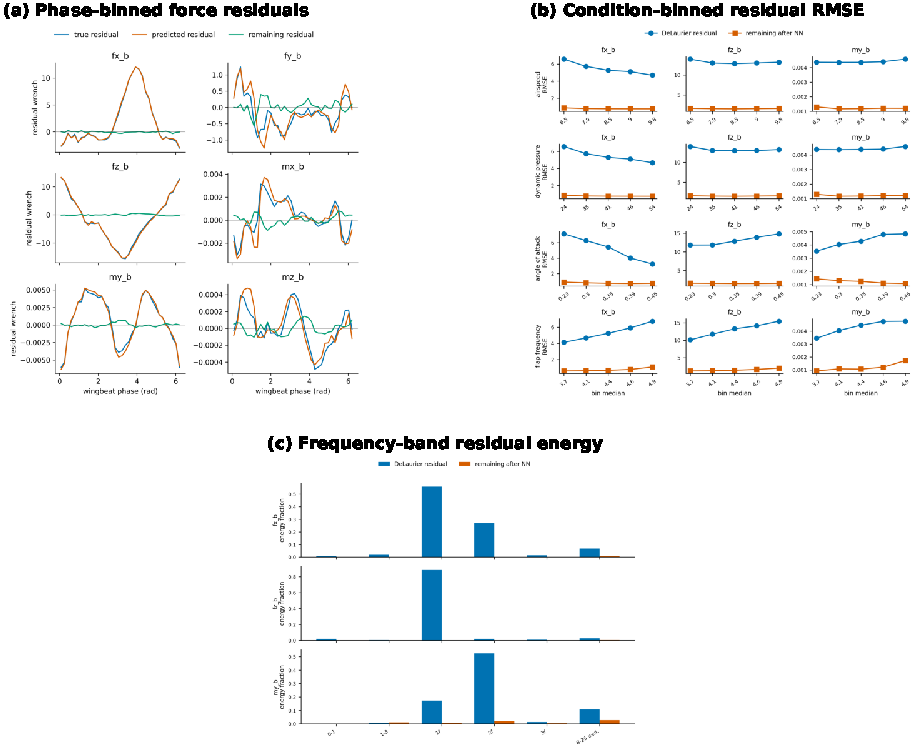
\includegraphics[width=\textwidth]{figures/residual_structure_summary.pdf}
  \caption{Force residual structure before and after neural correction. Panel (a) compares phase-binned median residuals. Panel (b) shows condition-binned residual RMSE. Panel (c) shows demeaned residual energy by frequency band; the shaded bars are remaining residual energy normalized by the original calibrated-model residual energy.}
  \label{fig:residual_structure}
\end{figure*}

\textit{Phase structure.} The main force-channel residuals contain repeatable wingbeat-phase waveforms, which indicates that the calibrated aerodynamic model leaves a cycle-synchronous mismatch rather than only random log noise. For $f_{x,b}$, phase-bin medians explain $0.817$ of the true residual variance and have a peak-to-peak amplitude of $15.10~\mathrm{N}$. For $f_{z,b}$, the corresponding phase $R^2$ is $0.509$ and the peak-to-peak amplitude is $28.79~\mathrm{N}$. The neural prediction follows these median waveforms closely, including the large positive $f_{x,b}$ residual during the latter half of the wingbeat and the sign-changing $f_{z,b}$ waveform over the cycle. After correction, the remaining phase peak-to-peak amplitudes fall to $0.56~\mathrm{N}$ and $0.98~\mathrm{N}$, respectively. This reduction is important because the model removes a repeatable intra-wingbeat component that the quasi-steady aerodynamic calculation does not capture.

\textit{Flight-condition dependence.} The force residual also varies across operating conditions, so the mismatch is not described completely by phase alone. The strongest dependence appears in $f_{x,b}$ versus angle of attack: residual RMSE changes by a factor of $2.21$ across bins, with the worst bin reaching $7.145~\mathrm{N}$. For $f_{z,b}$, the largest residual occurs at high angle of attack, reaching $14.809~\mathrm{N}$. Fig.~\ref{fig:residual_structure}(c) shows that the two force components have different trends with angle of attack: the calibrated model becomes less accurate in $f_{z,b}$ as angle of attack increases, while $f_{x,b}$ has larger residuals at the lower-angle bins in this flight envelope. Flapping frequency is also important: the highest-frequency bin reaches $6.735~\mathrm{N}$ in $f_{x,b}$ and $15.466~\mathrm{N}$ in $f_{z,b}$. The channel-aware hybrid model reduces the worst-bin errors to $0.896~\mathrm{N}$ and $2.059~\mathrm{N}$, respectively, but the remaining errors are not perfectly uniform across bins. This suggests that the learned correction is effective inside the observed envelope while still reflecting where the real-flight data provide more difficult or less repeated conditions.

\textit{Frequency-domain structure.} After subtracting segment means, most residual energy is organized around the flapping cycle. In $f_{x,b}$, $55.9\%$ of the residual energy is at the wingbeat fundamental and $26.9\%$ at the second harmonic. In $f_{z,b}$, the fundamental carries $88.4\%$ of the demeaned residual energy. These numbers are consistent with the phase-binned result: the force-model mismatch is dominated by repeatable periodic components, not by an arbitrary offset. The hybrid model removes nearly all of these components. In the dominant wingbeat-fundamental band, the remaining energy is only $0.27\%$ of the original band energy for $f_{x,b}$ and $0.13\%$ for $f_{z,b}$. Broadband high-frequency content is reduced less strongly, consistent with that band containing more sensor noise, effective-wrench reconstruction error, or nonrepeatable outdoor disturbance.

Together, these analyses show that the neural force residual is not merely lowering aggregate RMSE. It removes a structured discrepancy left by the calibrated aerodynamic model: a wingbeat-synchronous component, a flight-condition-dependent component, and a frequency-localized component. The remaining residual is therefore a more plausible mixture of unmodeled stochastic disturbance, label reconstruction noise, and operating points where the available flight logs provide weaker excitation.

\subsection{Interpretation and Limitations}
\label{subsec:interpretation_limitations}

The calibrated aerodynamic model provides a physically organized baseline. The
key result is that the force residual left by this baseline is stable and
interpretable. In the main force channels, the residual model mainly learns
wingbeat-synchronous correction. In the moment channels, the final model uses
direct neural prediction because the calibrated moment output is dominated by
large bias relative to the small measured moment range. The side-force channel
remains the most difficult force component, likely because of weaker lateral
excitation, wind disturbance, sideslip-estimation sensitivity, and label noise.

The residual should not be assigned to a single physical cause. It may reflect wing flexibility, unsteady loading, phase delay, actuator timing, tail/body coupling, airframe-specific parameters, or effective-wrench label reconstruction. The value of the residual analysis is narrower but still useful: it shows where the simulator prior is systematically mismatched and which parts of that mismatch can be learned from onboard measurements.

The present evaluation is log-based. It shows that the hybrid model predicts held-out effective wrench and removes structured force residual content, but it is not yet a closed-loop simulation validation. The next step is to embed the hybrid model in IsaacLab and evaluate short-horizon trajectory replay and controller performance. The dataset is also from one platform and a limited outdoor envelope, so future data should deliberately cover broader angle-of-attack, flapping-frequency, sideslip, and wind conditions, ideally with uncertainty estimates for out-of-envelope use.
